\documentclass[Second Project.tex]{subfiles}

\begin{document}
\subsection{ Μέθοδος \textlatin{Simpson} }
Η μέθοδος \textlatin{Simpson} προσεγγίζει την τιμή ενός ολοκληρώματος $\int_{a}^{b} f(x) \,dx$ μιας συνεχούς
συνάρτησης σε ένα κλειστό και φραγμένο διάστημα \textlatin{[a, b]} με χρήση εμβαδών παραβολών, οι οποίες 
προκύπτουν από την προσέγγιση της συνάρτησης $f$ σε στοιχειώδη υποδιαστήματα του \textlatin{[a, b]} από
πολυώνυμα 2ου βαθμού, δηλαδή από παραβολές. Η μέθοδος περιγράφεται παρακάτω
\begin{itemize}
    \item Έστω $\{x_{0}=a,\dots,x_{N}=b\}$, με $x_{0}<x_{1}<\dots<x_{N}$ ένας ομοιόμορφος διαμερισμός του
    \textlatin{[a, b]}, δηλαδή χωρίζουμε το \textlatin{[a, b]} σε \textit{Ν} ισομήκη υποδιαστήματα.
    \item Τότε $x_{i} = x_{0} + $κ$\frac{b-a}{N}$ ,  κ $=0,\dots,N$
    \item Υπολογίζουμε τις τιμές $f(x_{i}), i = 0,\dots,N$
    \item Σχηματίζουμε τις διαδοχικές παραβολές που διέρχονται από τα σημεία $f(x_{i}), \\ f(x_{i+1}), f(x_{i+2})$,
    $i = 0,\dots,N$, οπότε πρέπει Ν \textbf{ζυγός}.
    \item Υπολογίζουμε τα εμβαδά των Ν/2 παραβολών που σχηματίζονται και μετά από πράξεις έχουμε τελικά
\end{itemize} 
\begin{equation*}
    \int_{a}^{b} f(x) \,dx \approx \frac{b-a}{3N}(f(x_{0}) + f(x_{N}) + 2\sum_{i=1}^{\frac{N}{2}-1}f(x_{2i}) +
    4\sum_{i=1}^{\frac{N}{2}}f(x_{2i-1}) )
\end{equation*}
ενώ το άνω όριο του σφάλματος είναι
\begin{equation*}
    |e| \leq \frac{(b-a)^{5}}{180N^{4}}M ,
\end{equation*}
όπου
\begin{equation*}
M = max\{|f^{(4)}(x)|: x\in \textlatin{[a, b]}\}
\end{equation*}

Στο αρχείο \textlatin{\textbf{simpson.py}} έχουν αναπτυχθεί δύο συναρτήσεις, μία για τον υπολογισμό ενός ολοκληρώματος
από το $a$ στο $b$ για μία συνεχή συνάρτηση $f$ με την μέθοδο \textlatin{Simpson}, καθώς και μία για τον υπολογισμό του
άνω ορίου του σφάλματος για τις προαναφερόμενες παραμέτρους. Αν καλέσουμε την συνάρτηση 
\textit{\textlatin{\textbf{simpson\_integrate}}} με ορίσματα την συνάρτηση του ημιτόνου, το 0, το $\frac{\pi}{2}$, το 10 
και τα σημεία που αναφέρθηκαν στην εισαγωγή αυτής της άσκησης, καθώς και την συνάρτηση 
\textlatin{\textbf{\textbf{simpson\_error\_bound}}} με τα ίδια ορίσματα εκτός της λίστας των σημείων λαμβάνουμε τα παρακάτω
\begin{figure}[h!]
    \centering
    \captionsetup{justification=centering}
    \begin{center}
    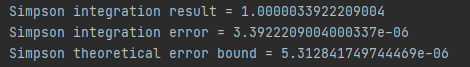
\includegraphics[scale=1]{simpson_results.png}    
    \caption{ Αποτελέσματα κλήσης της συνάρτησης \textit{\textlatin{\textbf{simpson\_integrate}}} 
    και \textit{\textlatin{\textbf{simpson\_error\_bound}}} στο διάστημα $[0, \frac{\pi}{2}]$.}
    \end{center}
\end{figure}

Απ' όπου παρατηρούμε ότι το σφάλμα προσέγγισης θεωρητικά είναι \\ $5.312841749744469e-06$ ενώ αριθμητικά ( δηλαδή 
αφαιρώντας από την πραγματική τιμή του ολοκληρώματος, που είναι 1, και εφαρμόζοντας απόλυτη τιμή ) είναι
$3.3922209004000337e-06$ και τέλος, η προσεγγιστική τιμή του ολοκληρώματος με την μέθοδο \textlatin{\textbf{Simpson}}
είναι $1.0000033922209004$. 
\end{document}